\documentclass[14pt]{extbook}
\usepackage{multicol, enumerate, enumitem, hyperref, color, soul, setspace, parskip, fancyhdr} %General Packages
\usepackage{amssymb, amsthm, amsmath, latexsym, units, mathtools} %Math Packages
\everymath{\displaystyle} %All math in Display Style
% Packages with additional options
\usepackage[headsep=0.5cm,headheight=12pt, left=1 in,right= 1 in,top= 1 in,bottom= 1 in]{geometry}
\usepackage[usenames,dvipsnames]{xcolor}
\usepackage{dashrule}  % Package to use the command below to create lines between items
\newcommand{\litem}[1]{\item#1\hspace*{-1cm}\rule{\textwidth}{0.4pt}}
\pagestyle{fancy}
\lhead{Progress Quiz 7}
\chead{}
\rhead{Version C}
\lfoot{3510-5252}
\cfoot{}
\rfoot{Summer C 2021}
\begin{document}

\begin{enumerate}
\litem{
Choose the equation of the function graphed below.
\begin{center}
    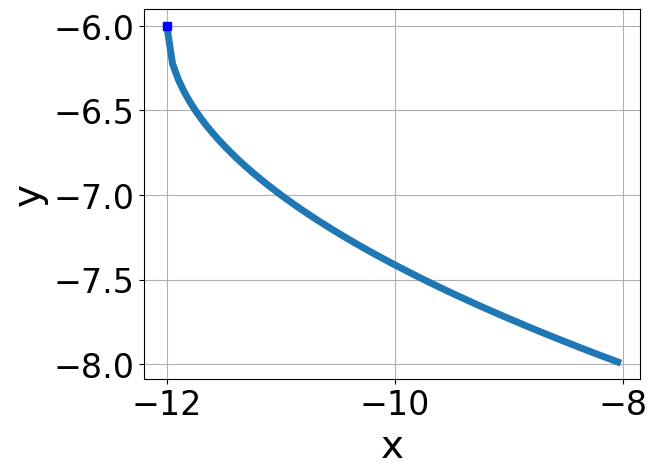
\includegraphics[width=0.5\textwidth]{../Figures/radicalGraphToEquationCopyC.png}
\end{center}
\begin{enumerate}[label=\Alph*.]
\item \( f(x) = \sqrt{x - 12} - 6 \)
\item \( f(x) = - \sqrt{x - 12} - 6 \)
\item \( f(x) = \sqrt{x + 12} - 6 \)
\item \( f(x) = - \sqrt{x + 12} - 6 \)
\item \( \text{None of the above} \)

\end{enumerate} }
\litem{
Choose the graph of the equation below.\[ f(x) = - \sqrt[3]{x + 14} + 4 \]\begin{enumerate}[label=\Alph*.]
\begin{multicols}{2}\item 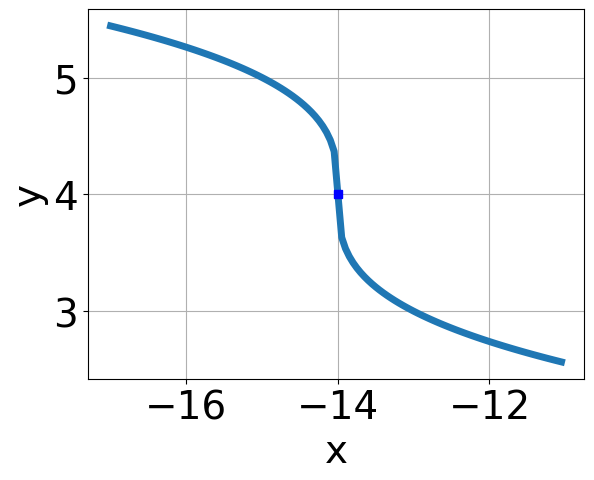
\includegraphics[width = 0.3\textwidth]{../Figures/radicalEquationToGraphAC.png}\item 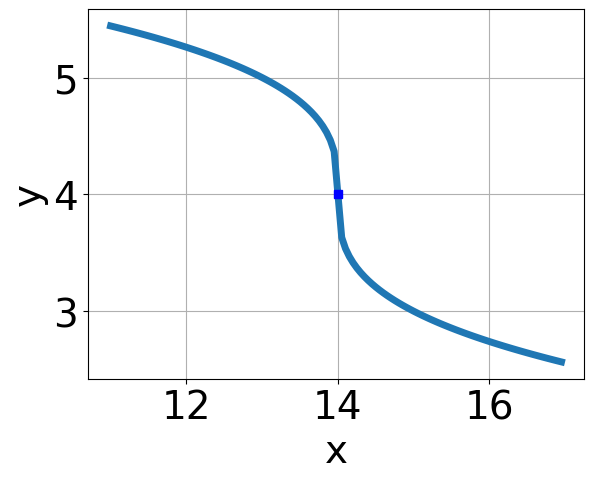
\includegraphics[width = 0.3\textwidth]{../Figures/radicalEquationToGraphBC.png}\item 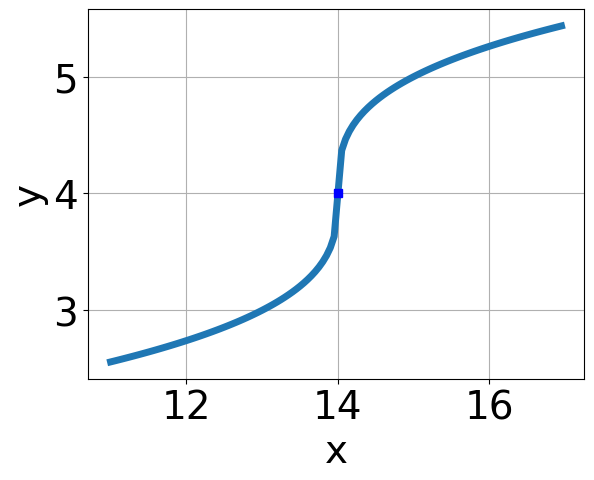
\includegraphics[width = 0.3\textwidth]{../Figures/radicalEquationToGraphCC.png}\item 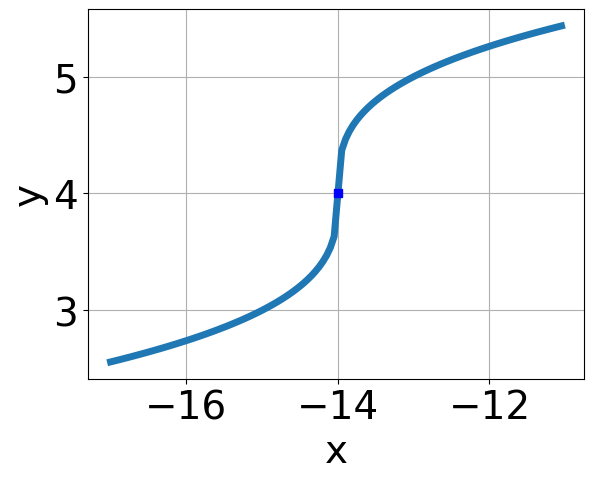
\includegraphics[width = 0.3\textwidth]{../Figures/radicalEquationToGraphDC.png}\end{multicols}\item None of the above.
\end{enumerate} }
\litem{
Solve the radical equation below. Then, choose the interval(s) that the solution(s) belongs to.\[ \sqrt{-40 x^2 + 8} - \sqrt{-4 x} = 0 \]\begin{enumerate}[label=\Alph*.]
\item \( \text{All solutions lead to invalid or complex values in the equation.} \)
\item \( x \in [0.42,0.5] \)
\item \( x \in [-0.56,-0.3] \)
\item \( x_1 \in [-0.56, -0.3] \text{ and } x_2 \in [-5.5,4.5] \)
\item \( x_1 \in [0.35, 0.45] \text{ and } x_2 \in [-5.5,4.5] \)

\end{enumerate} }
\litem{
Choose the equation of the function graphed below.
\begin{center}
    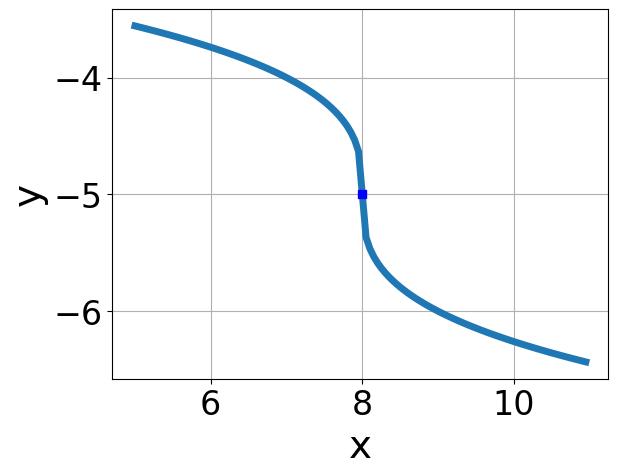
\includegraphics[width=0.5\textwidth]{../Figures/radicalGraphToEquationC.png}
\end{center}
\begin{enumerate}[label=\Alph*.]
\item \( f(x) = \sqrt[3]{x - 8} - 5 \)
\item \( f(x) = \sqrt[3]{x + 8} - 5 \)
\item \( f(x) = - \sqrt[3]{x - 8} - 5 \)
\item \( f(x) = - \sqrt[3]{x + 8} - 5 \)
\item \( \text{None of the above} \)

\end{enumerate} }
\litem{
Solve the radical equation below. Then, choose the interval(s) that the solution(s) belongs to.\[ \sqrt{10 x^2 + 45} - \sqrt{-55 x} = 0 \]\begin{enumerate}[label=\Alph*.]
\item \( \text{All solutions lead to invalid or complex values in the equation.} \)
\item \( x \in [-5.6,-3.1] \)
\item \( x \in [-1.1,0.1] \)
\item \( x_1 \in [-5.6, -3.1] \text{ and } x_2 \in [-4,1] \)
\item \( x_1 \in [0.2, 1.3] \text{ and } x_2 \in [0.5,6.5] \)

\end{enumerate} }
\litem{
Solve the radical equation below. Then, choose the interval(s) that the solution(s) belongs to.\[ \sqrt{-4 x - 8} - \sqrt{5 x - 6} = 0 \]\begin{enumerate}[label=\Alph*.]
\item \( x \in [-0.92,1.18] \)
\item \( x_1 \in [-2.87, -1.88] \text{ and } x_2 \in [1,2.4] \)
\item \( x \in [-1.86,-1.48] \)
\item \( \text{All solutions lead to invalid or complex values in the equation.} \)
\item \( x_1 \in [-2.87, -1.88] \text{ and } x_2 \in [-0.9,0.9] \)

\end{enumerate} }
\litem{
What is the domain of the function below?\[ f(x) = \sqrt[4]{-5 x + 8} \]\begin{enumerate}[label=\Alph*.]
\item \( [a, \infty), \text{where } a \in [0, 1] \)
\item \( (-\infty, a], \text{where } a \in [-1.3, 1.2] \)
\item \( (-\infty, \infty) \)
\item \( (-\infty, a], \text{ where } a \in [1.3, 5.9] \)
\item \( [a, \infty), \text{where } a \in [1.1, 4.5] \)

\end{enumerate} }
\litem{
Choose the graph of the equation below.\[ f(x) = \sqrt{x - 10} + 7 \]\begin{enumerate}[label=\Alph*.]
\begin{multicols}{2}\item 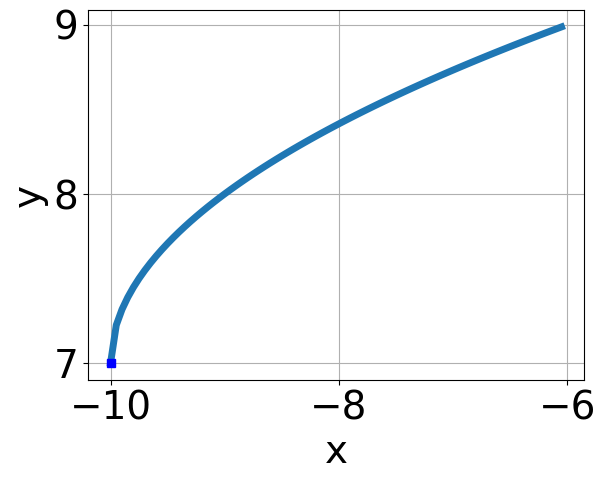
\includegraphics[width = 0.3\textwidth]{../Figures/radicalEquationToGraphCopyAC.png}\item 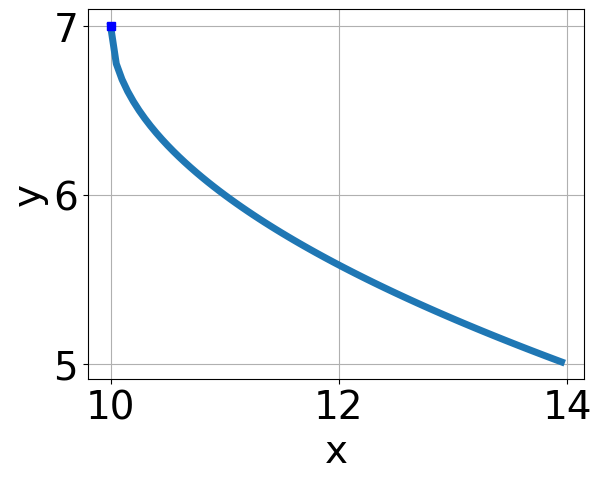
\includegraphics[width = 0.3\textwidth]{../Figures/radicalEquationToGraphCopyBC.png}\item 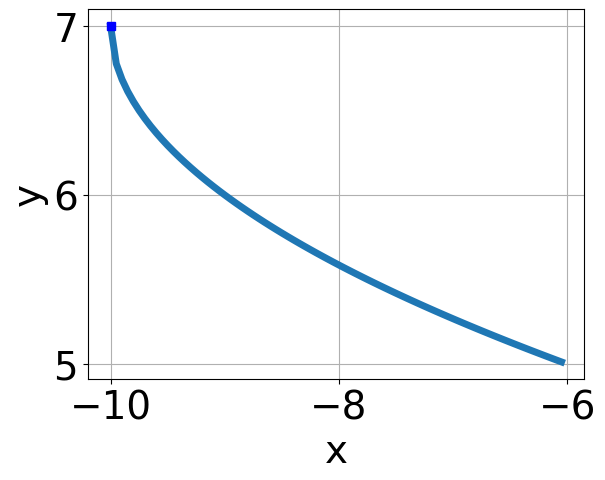
\includegraphics[width = 0.3\textwidth]{../Figures/radicalEquationToGraphCopyCC.png}\item 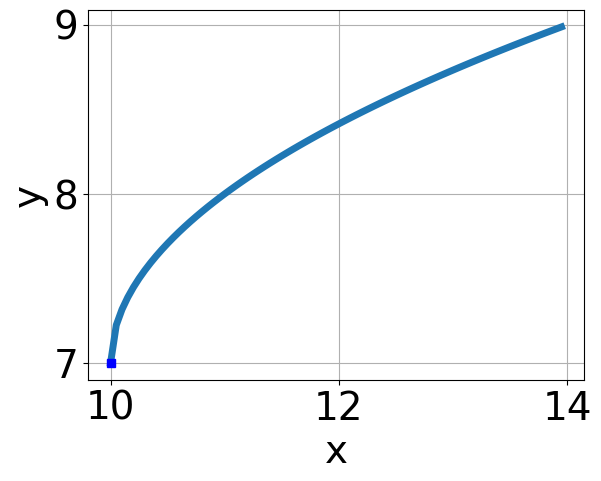
\includegraphics[width = 0.3\textwidth]{../Figures/radicalEquationToGraphCopyDC.png}\end{multicols}\item None of the above.
\end{enumerate} }
\litem{
What is the domain of the function below?\[ f(x) = \sqrt[5]{3 x - 9} \]\begin{enumerate}[label=\Alph*.]
\item \( \text{The domain is } [a, \infty), \text{   where } a \in [0.3, 1.6] \)
\item \( \text{The domain is } (-\infty, a], \text{   where } a \in [-1.67, 2.33] \)
\item \( \text{The domain is } [a, \infty), \text{   where } a \in [1.6, 6.1] \)
\item \( (-\infty, \infty) \)
\item \( \text{The domain is } (-\infty, a], \text{   where } a \in [2, 5] \)

\end{enumerate} }
\litem{
Solve the radical equation below. Then, choose the interval(s) that the solution(s) belongs to.\[ \sqrt{9 x + 8} - \sqrt{7 x + 2} = 0 \]\begin{enumerate}[label=\Alph*.]
\item \( x_1 \in [-3.06, -2.66] \text{ and } x_2 \in [-1.29,-0.58] \)
\item \( x \in [-3.06,-2.66] \)
\item \( x \in [-5.14,-3.53] \)
\item \( \text{All solutions lead to invalid or complex values in the equation.} \)
\item \( x_1 \in [-1.31, 0.27] \text{ and } x_2 \in [-0.54,0.15] \)

\end{enumerate} }
\end{enumerate}

\end{document}